\documentclass[sigconf]{acmart}
\usepackage{lipsum} 

\settopmatter{printacmref=false} % Removes citation information below abstract
\renewcommand\footnotetextcopyrightpermission[1]{}
\pagestyle{plain} % removes running headers

%%
%% \BibTeX command to typeset BibTeX logo in the docs
\AtBeginDocument{%
  \providecommand\BibTeX{{%
    Bib\TeX}}}

\setcopyright{None}

\settopmatter{printacmref=false}

\begin{document}

\title{The Name of the Title Is Hope}

\author{Sofiane Ezzehi}
\affiliation{%
  \institution{Ecole Normale Supérieure Paris-Saclay \\ Ecole des Ponts ParisTech}
  \country{}
}
\email{sofiane.ezzehi@eleves.enpc.fr}

\author{Alexandre Lutt}
\affiliation{%
  \institution{Ecole Normale Supérieure Paris-Saclay \\ Ecole des Ponts ParisTech}
  \country{}
}
\email{alexandre.lutt@eleves.enpc.fr}

\begin{teaserfigure}
  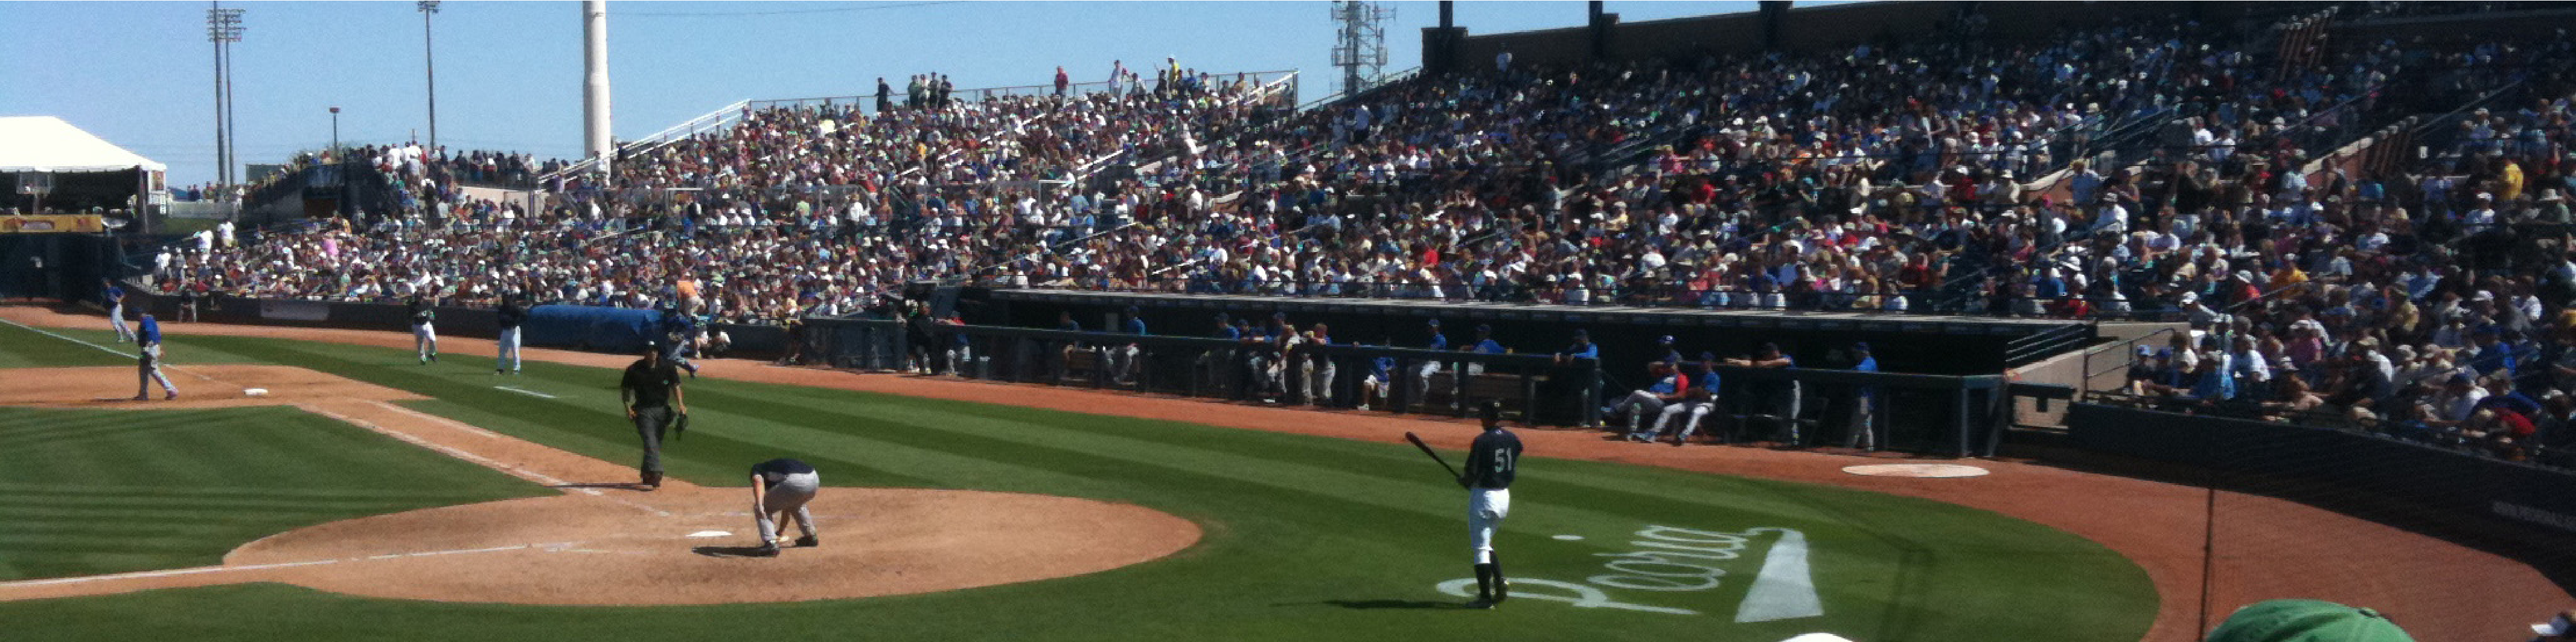
\includegraphics[width=\textwidth]{sampleteaser}
  \caption{Seattle Mariners at Spring Training, 2010.}
  \Description{Enjoying the baseball game from the third-base
  seats. Ichiro Suzuki preparing to bat.}
  \label{fig:teaser}
\end{teaserfigure}

\maketitle
\pagestyle{plain}

\section{Introduction}

\lipsum[1]~\cite{main_paper}

\lipsum[1]~\cite{rpca_paper}

%%
%% The next two lines define the bibliography style to be used, and
%% the bibliography file.
\bibliographystyle{ACM-Reference-Format}
\bibliography{bib}

\end{document}
\endinput